\documentclass[tikz,border=5pt]{standalone}
\usepackage{luatexja}
\usepackage[hiragino-pron]{luatexja-preset}
\usepackage{amsmath,amssymb,bm}
\usetikzlibrary{arrows.meta}

\begin{document}
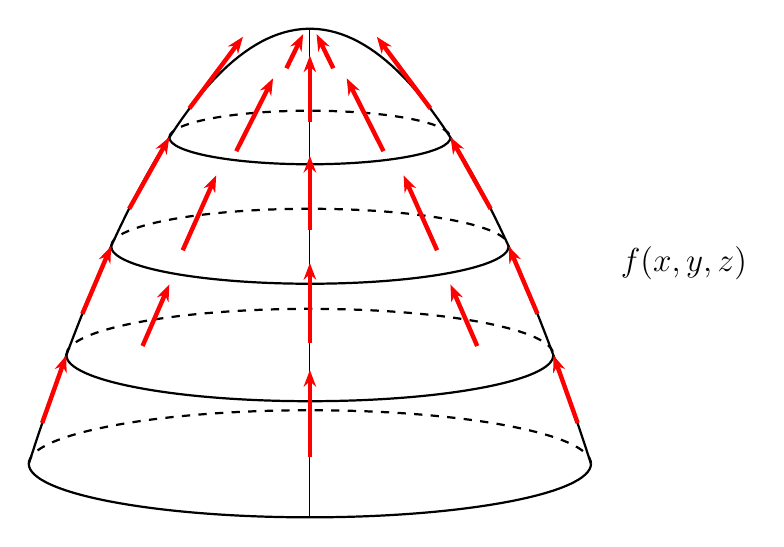
\begin{tikzpicture}[every node/.style={font=\large}, scale=0.85]

  % Paraboloid outline: z = 6.5*(1 - (x/4.2)^2), flat top, parabolic sides
  \draw[thick, domain=-4.2:4.2, samples=100]
    plot (\x, {6.5*(1 - (\x/4.2)^2)});

  % Contour ellipses at heights z = 0, 1.625, 3.25, 4.875
  % Radius from paraboloid: r = 4.2*sqrt(1 - z/6.5)
  % z=0:     r=4.2*1       = 4.20,  ry=0.80
  % z=1.625: r=4.2*sqrt(3/4)= 3.64, ry=0.69
  % z=3.25:  r=4.2*sqrt(1/2)= 2.97, ry=0.56
  % z=4.875: r=4.2*sqrt(1/4)= 2.10, ry=0.40

  % Bottom ellipse (z=0)
  \draw[thick] (-4.2,0) arc[start angle=180, end angle=360, x radius=4.2, y radius=0.8];
  \draw[thick, dashed] (-4.2,0) arc[start angle=180, end angle=0, x radius=4.2, y radius=0.8];

  % Contour ellipse at z=1.625
  \draw[thick] (-3.64,1.625) arc[start angle=180, end angle=360, x radius=3.64, y radius=0.69];
  \draw[thick, dashed] (-3.64,1.625) arc[start angle=180, end angle=0, x radius=3.64, y radius=0.69];

  % Contour ellipse at z=3.25
  \draw[thick] (-2.97,3.25) arc[start angle=180, end angle=360, x radius=2.97, y radius=0.56];
  \draw[thick, dashed] (-2.97,3.25) arc[start angle=180, end angle=0, x radius=2.97, y radius=0.56];

  % Contour ellipse at z=4.875
  \draw[thick] (-2.1,4.875) arc[start angle=180, end angle=360, x radius=2.1, y radius=0.4];
  \draw[thick, dashed] (-2.1,4.875) arc[start angle=180, end angle=0, x radius=2.1, y radius=0.4];

  % Central axis
  \draw[thin] (0,-0.8) -- (0,6.5);

  % Gradient arrows on the parabola z = 6.5*(1 - (x/4.2)^2)
  % Each arrow starts and ends ON the curve

  % Left slope
  \draw[-{Stealth[length=6pt]}, ultra thick, red] (-4.0,0.61) -- (-3.64,1.62);
  \draw[-{Stealth[length=6pt]}, ultra thick, red] (-3.4,2.24) -- (-2.97,3.25);
  \draw[-{Stealth[length=6pt]}, ultra thick, red] (-2.7,3.81) -- (-2.1,4.88);
  \draw[-{Stealth[length=6pt]}, ultra thick, red] (-1.8,5.31) -- (-1.0,6.38);

  % Center
  \draw[-{Stealth[length=6pt]}, ultra thick, red] (0,0.1) -- (0,1.4);
  \draw[-{Stealth[length=6pt]}, ultra thick, red] (0,1.8) -- (0,3.0);
  \draw[-{Stealth[length=6pt]}, ultra thick, red] (0,3.5) -- (0,4.6);
  \draw[-{Stealth[length=6pt]}, ultra thick, red] (0,5.1) -- (0,6.1);

  % Inner left slope (shifted slightly right)
  \draw[-{Stealth[length=6pt]}, ultra thick, red] (-2.5,1.76) -- (-2.1,2.68);
  \draw[-{Stealth[length=6pt]}, ultra thick, red] (-1.9,3.19) -- (-1.4,4.31);
  \draw[-{Stealth[length=6pt]}, ultra thick, red] (-1.1,4.67) -- (-0.55,5.76);
  \draw[-{Stealth[length=6pt]}, ultra thick, red] (-0.35,5.91) -- (-0.1,6.42);

  % Inner right slope (shifted slightly left)
  \draw[-{Stealth[length=6pt]}, ultra thick, red] (2.5,1.76) -- (2.1,2.68);
  \draw[-{Stealth[length=6pt]}, ultra thick, red] (1.9,3.19) -- (1.4,4.31);
  \draw[-{Stealth[length=6pt]}, ultra thick, red] (1.1,4.67) -- (0.55,5.76);
  \draw[-{Stealth[length=6pt]}, ultra thick, red] (0.35,5.91) -- (0.1,6.42);

  % Right slope
  \draw[-{Stealth[length=6pt]}, ultra thick, red] (4.0,0.61) -- (3.64,1.62);
  \draw[-{Stealth[length=6pt]}, ultra thick, red] (3.4,2.24) -- (2.97,3.25);
  \draw[-{Stealth[length=6pt]}, ultra thick, red] (2.7,3.81) -- (2.1,4.88);
  \draw[-{Stealth[length=6pt]}, ultra thick, red] (1.8,5.31) -- (1.0,6.38);

  % Label
  \node[right] at (4.5,3) {$f(x, y, z)$};

\end{tikzpicture}
\end{document}
